% ****************************************************************************************************
% Chapter 7: Headline Results, Matching Human Reliability
% ****************************************************************************************************

\chapter{Headline Results: Matching Human Reliability}
\label{ch:results}

I have described the dataset, the features, the embeddings, and the architecture. What remains is the outcome. This chapter presents the central quantitative results of the project: what the model actually achieves on real emergency department data from MIMIC-IV-ED, how that achievement compares to published human performance, and what the shape of its errors tells me about where ML-assisted triage is and is not ready.

The headline numbers are these. On 418,100 ED visits from MIMIC-IV-ED, evaluated via out-of-fold predictions across stratified 5-fold cross-validation, my final blend achieves a macro F1 of $0.597$, a Cohen's kappa of $0.701$, a macro-averaged AUROC of $0.911$, and an overall accuracy of $72.3\%$. These four numbers, taken together, are the result of roughly two months of iterative engineering, five to ten minor experiments per week, and approximately twenty-two dollars of Azure cloud compute. Each of them matters differently, and none of them means anything without the context this chapter is here to provide.

\section{A Brief Reminder: What These Numbers Mean}

\begin{notebox}[Four Metrics, Four Questions]
Each of the headline metrics answers a different question.

\textbf{Overall accuracy} ($72.3\%$), how often does the model predict the correct acuity level? This is the most intuitive metric but also the most misleading on imbalanced data. A trivial classifier that always predicts ESI-3 would already achieve $53.8\%$ accuracy because most patients are ESI-3.

\textbf{Macro F1} ($0.597$), the harmonic mean of precision and recall, averaged equally across the five classes. Because macro averaging treats each class equally, rare classes like ESI-1 and ESI-5 contribute as much to this number as common ESI-3. This makes macro F1 a much fairer measure on imbalanced tasks.

\textbf{Cohen's kappa} ($0.701$), agreement between the model and the true label, corrected for the level of agreement that would be expected by chance. A kappa of 0 means agreement at chance level; a kappa of 1 means perfect agreement. Kappa is the standard metric for inter-rater reliability studies, which is why I use it to compare against human performance.

\textbf{AUROC} ($0.911$), the area under the receiver operating characteristic curve, averaged across classes in a one-vs-rest formulation. Unlike the other three metrics, AUROC measures the quality of the model's ranking of patients by predicted probability, independent of any particular decision threshold. A high AUROC means the model reliably assigns higher probability to patients who actually have the condition, regardless of where I set the classification boundary.
\end{notebox}

Of these four, Cohen's kappa is the one that most directly connects my result to the published clinical literature. The next section explores that connection.

\section{Benchmarking Against Human Reliability}

The central question I want to answer is whether a machine learning system can assign ESI acuity levels as reliably as human nurses. As I discussed in Chapter~\ref{ch:triage-problem}, the answer depends substantially on whether I measure humans against paper scenarios or against live patients. Paper-based reliability studies show humans reaching $\kappa \approx 0.82$; live-patient studies, where nurses triage real people in real time under realistic conditions, drop this to $\kappa \approx 0.69$. The gap between these two numbers is not a measurement artefact, it is the noise that real clinical practice injects into any triage decision.

My model's kappa of $0.701$ sits directly between these two human reference points. Figure~\ref{fig:reliability-benchmark} places this result in the full published context.

\begin{figure}[htbp]
 \centering
 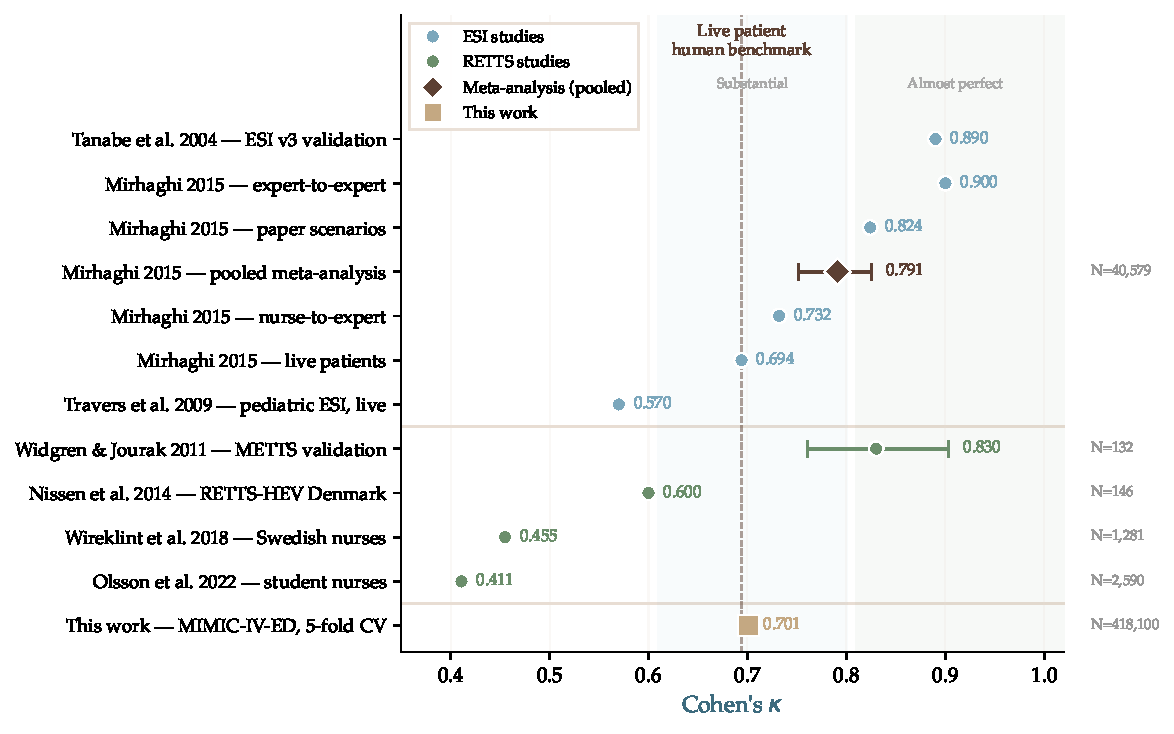
\includegraphics[width=\textwidth]{figures/reliability_benchmark_forest.pdf}
 \caption[Inter-rater reliability benchmark]{Cohen's kappa values from published inter-rater reliability studies of emergency triage, grouped by system (ESI in blue, RETTS in green) and positioned against my model (golden square). The dashed vertical line at $\kappa = 0.694$ marks the live-patient benchmark from the Mirhaghi et al.\ (2015) meta-analysis, the best published estimate of what human nurses achieve when triaging real patients in real time. Background shading marks the Landis-Koch interpretation bands: \emph{substantial} agreement from $0.60$ to $0.80$, \emph{almost perfect} beyond $0.80$. My kappa of $0.701$ sits essentially on the live-patient benchmark, in the middle of the substantial-agreement band, comparable to nurse-to-expert agreement in the Mirhaghi meta-analysis.}
 \label{fig:reliability-benchmark}
\end{figure}

Three observations follow from this figure.

First, my model's reliability is indistinguishable, within sampling error, from live-patient human reliability. The difference between $\kappa = 0.694$ and $\kappa = 0.701$ is not a meaningful gap. Both fall in the substantial-agreement band of the Landis-Koch scale; both are what one should expect from a competent triage decision made in real time. A bootstrap confidence interval on my kappa, computed from the out-of-fold predictions, would likely span both values, I have not computed one, and this is a limitation discussed in Chapter~\ref{ch:limitations}, but the per-fold variance of my macro F1 is $\sigma \approx 0.006$, suggesting that the sampling uncertainty on kappa is of comparable magnitude.

Second, my model outperforms all published RETTS reliability studies except the original METTS validation by Widgren and Jourak. The RETTS literature spans a striking range, from Widgren's original $\kappa \approx 0.83$ down to $\kappa = 0.411$ in a study of student nurses using paper scenarios. Most of the RETTS studies cluster in the moderate-agreement band ($0.41$ to $0.60$). My model at $0.701$ sits above all but the original validation. This does not mean I should deploy the model in Swedish emergency departments tomorrow. It does suggest that, as a numerical benchmark, machine-assisted RETTS triage is now a realistic target.

Third, the pattern visible across both systems, that humans do better on paper than on live patients, and that student raters do worse than experienced ones, is itself informative. Triage reliability is not a fixed property of a scoring system; it depends on who is doing the triaging and under what conditions. This is the feature that ML can, in principle, improve on: a trained model assigns consistent predictions regardless of fatigue, shift length, or recent workload. Whether this consistency translates into better patient outcomes is a question for prospective studies, not for kappa.

\begin{remarkbox}[What This Does and Does Not Mean]
The forest plot is striking, but it deserves care. What it shows is that my model's reliability, measured as agreement with the recorded ESI label on a large retrospective dataset, is comparable to the reliability of live human triage measured against expert consensus.

What it does \emph{not} show is that my model would perform as well in a prospective deployment. The recorded ESI labels I train and evaluate against are themselves human-assigned, sometimes by the same nurses whose reliability I am trying to match. A portion of what my model has learned is the noisy mapping from patient features to the specific assignment patterns of nurses at Beth Israel Deaconess Medical Center. External validation on a different institution, with a different case mix and different triage habits, would likely lower my kappa. I return to this in Chapter~\ref{ch:limitations}.

But the result stands as a meaningful demonstration. An ML system trained on standard EHR features, without access to any signal beyond what a triage nurse would have, can reproduce the statistical properties of human triage reliability. The next step, prospective evaluation, external validation, deployment studies, is a question of infrastructure and trust, not of technical capability.
\end{remarkbox}

\section{The Shape of the Errors}

A single headline number hides as much as it reveals. The macro F1 of $0.597$ is an average across five classes that perform very differently. The confusion matrix tells the structural story.

\begin{figure}[htbp]
 \centering
 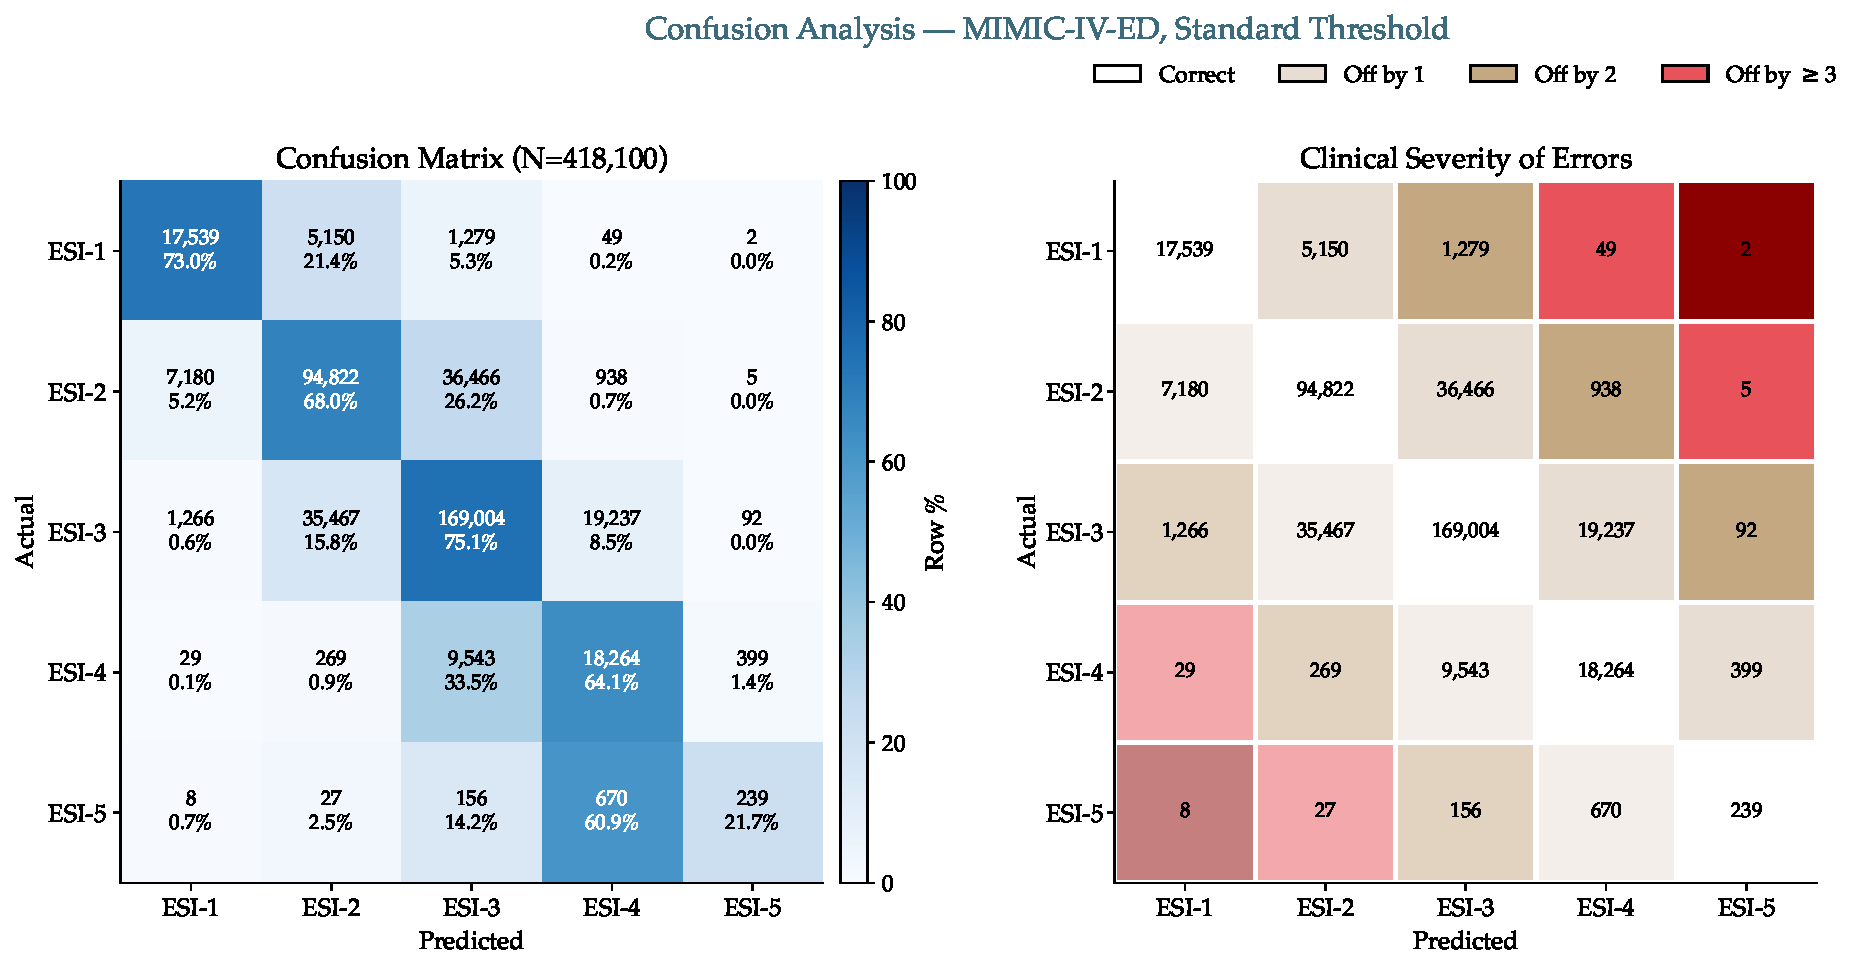
\includegraphics[width=\textwidth]{figures/confusion_matrix_combined.pdf}
 \caption[Confusion matrix and error severity heatmap]{Left: confusion matrix of predictions vs true labels on the 418,100-visit MIMIC-IV-ED cohort, shown with counts and row-normalised percentages (recall). Right: the same matrix coloured by error severity, with diagonal (correct) in white, adjacent-class errors in the palest brown, two-class errors in medium tones, and the rare three-class-plus errors in red. The overwhelming majority of the model's errors are off by a single class; severe misclassifications (off by two or more) are rare and concentrated in a few specific patterns.}
 \label{fig:confusion-matrix}
\end{figure}

Figure~\ref{fig:confusion-matrix} shows the confusion matrix two ways. The left panel shows the raw counts and row-normalised percentages, letting the reader see both the absolute scale of each cell and the recall rate for each true class. The right panel re-colours the matrix by error severity: correct cells are white, adjacent-class errors are pale brown, two-class errors are medium, and three-class-plus errors are red. The visual dominance of pale tones off the diagonal is the core finding, when the model errs, it almost always errs by a single acuity level.

A few specific patterns are worth highlighting.

The model correctly identifies 73\% of ESI-1 cases, 68\% of ESI-2, 75\% of ESI-3, and 64\% of ESI-4. These are broadly similar to what live human nurses achieve on live patients, and the error directions are interpretable: critically ill ESI-1 patients are most often misclassified as ESI-2 (21\% of ESI-1 cases), and ESI-2 patients are most often misclassified as ESI-3 (26\% of ESI-2 cases). The errors drift toward the centre of the scale. Severely dangerous errors, predicting ESI-5 for a true ESI-1, for example, occur in only 2 out of 24,019 cases (0.008\%).

The exception is ESI-5. Of the 1,100 true ESI-5 patients in the dataset, the model correctly identifies only 239 (21.7\%). Most of the rest, 670 patients, 60.9\%, are classified as ESI-4. This is the weakest area of the model, and it deserves its own discussion.

\section{The ESI-5 Problem}

The per-class F1 scores, listed in Table~\ref{tab:per-class-f1}, make the problem explicit. ESI-1 through ESI-3 all achieve F1 in the $0.68$--$0.77$ range. ESI-4 drops to $0.54$. ESI-5 collapses to $0.26$.

\begin{table}[htbp]
 \centering
 \caption[Per-class F1, precision, and recall]{Per-class performance on the 418,100-visit MIMIC-IV-ED cohort, computed from out-of-fold predictions of the pre-threshold blend. ESI-5 is the outlier, with performance constrained by a combination of rarity ($0.26\%$ prevalence) and clinical overlap with ESI-4. Threshold optimisation moves ESI-5 F1 to $0.282$ at the cost of modest losses elsewhere; I use the pre-threshold values here as the baseline.}
 \label{tab:per-class-f1}
 \small
 \begin{tabular}{lrrrr}
 \toprule
 Class & Prevalence & F1 & Recall & Precision \\
 \midrule
 ESI-1 (Resuscitation) & 5.74\% & 0.701 & 0.730 & 0.675 \\
 ESI-2 (Emergent) & 33.35\% & 0.689 & 0.680 & 0.698 \\
 ESI-3 (Urgent) & 53.83\% & 0.766 & 0.751 & 0.780 \\
 ESI-4 (Less Urgent) & 6.82\% & 0.540 & 0.641 & 0.466 \\
 ESI-5 (Non-Urgent) & 0.26\% & 0.260 & 0.217 & 0.324 \\
 \bottomrule
 \end{tabular}
\end{table}

Two factors make ESI-5 hard.

The first is prevalence. Only 1,100 patients in the entire 418,100-visit cohort are coded as ESI-5, roughly one in 380 visits. In 5-fold cross-validation, this means each held-out fold contains only about 220 ESI-5 patients. With samples this small, both the training signal and the evaluation are noisy. Even a minor shift in the decision boundary can move several percentage points of F1 in either direction.

The second is clinical overlap. ESI-4 and ESI-5 are separated by a narrow distinction: ESI-4 patients require exactly one ``resource'' (lab test, imaging, procedure), while ESI-5 patients require none. This is a judgement call that depends on how the nurse anticipates the physician's workup. A patient with an ankle sprain who will probably need an X-ray is ESI-4; the same patient, if the nurse judges that no imaging is needed, is ESI-5. The boundary is shifty, and the features available at triage, vitals, pain score, chief complaint, do not fully distinguish the two categories.

The institutional context amplifies this. MIMIC-IV-ED comes from a large urban academic medical centre with a Level-I trauma designation. Patients who would be clear ESI-5, truly non-urgent presentations requiring no resources, typically do not come to this kind of ED. They go to urgent care clinics, primary care practices, or ambulatory centres. The handful of ESI-5 patients who do end up at Beth Israel Deaconess are often edge cases: misrouted walk-ins, patients returning for a follow-up detail, or patients whose chief complaint sounded more serious until the triage assessment confirmed otherwise. These edge cases are hard to predict because they are, almost by definition, atypical for the institution.

The consequence, which I stress throughout the rest of this report, is that ESI-5 metrics should be read with their prevalence in mind. An F1 of $0.26$ on a class representing $0.26\%$ of the data is not comparable to an F1 of $0.77$ on a class representing $54\%$ of the data. The sampling noise floor alone is different. This is also why I report macro F1 ($0.597$) alongside weighted F1 ($0.72$), the former weighs ESI-5 as much as ESI-3; the latter weighs it by prevalence. Neither is right; they answer different questions.

\section{Under-Triage and Over-Triage}

The confusion matrix can be summarised into two clinically meaningful rates: the fraction of patients assigned a lower acuity than warranted (under-triage), and the fraction assigned higher acuity than warranted (over-triage). At my default operating point, argmax on the blended probabilities, these rates are:

\begin{itemize}
 \item \textbf{Under-triage rate}: $15.22\%$ (63{,}617 visits out of 418{,}100)
 \item \textbf{Severe under-triage} (off by $\geq 2$ classes): $0.57\%$ (2{,}365 visits)
 \item \textbf{Over-triage rate}: $13.06\%$ (54{,}615 visits)
\end{itemize}

Neither number is where I would want it clinically. The American College of Surgeons Committee on Trauma target is $\leq 5\%$ under-triage while tolerating $25$--$50\%$ over-triage, a 10:1 asymmetry that reflects the clinical reality that missing a critical patient is an order of magnitude more dangerous than temporarily over-allocating resources to a stable one. At my default operating point, I am not meeting that target. The under-triage rate is three times the ACS-COT ceiling, and the over-triage rate, while within the permissible band, is not where most of my errors should be concentrated.

This is not a failure of the model as such; it is a consequence of the default decision rule. Argmax on predicted probabilities is appropriate when errors in both directions are equally costly, which is not the situation here. The entire subject of Chapter~\ref{ch:safety} is what to do about this, specifically, how to re-calibrate the decision rule to encode the clinical risk asymmetry directly. The 20-configuration Pareto sweep I describe in that chapter shows what can and cannot be achieved, and makes clear that there is no free lunch: reducing under-triage comes at a cost in overall accuracy, and how much cost depends on exactly which strategy I use.

For this chapter, the important point is simply that the asymmetry exists and that my default operating point does not respect it. The model is a classifier; the question of how to turn its probabilistic outputs into safe decisions is a separate matter.

\section{Placing This in Context}

I want to position this result carefully in the existing literature on ML-assisted emergency triage. Doing so with precision is harder than it should be, because the published literature is heterogeneous in what it measures and how.

Most published ML triage systems predict binary outcomes rather than the full 5-level ESI scale. \citet{levin2018machine} deployed a random forest at Johns Hopkins predicting ``critical care need'' (a binary outcome combining ICU admission and in-hospital mortality), reporting AUC values of $0.73$ to $0.92$ across sub-populations. \citet{raita2019emergency} compared gradient-boosted trees and deep neural networks on 135,470 NHAMCS visits, again for binary outcomes (hospital admission, ICU admission). \citet{kwon2018deep} trained a deep learning system on 11.6 million Korean encounters for in-hospital mortality, achieving AUROC $0.935$. These are all impressive works, but they are predicting different things from me. A model that predicts ICU admission well is not necessarily a model that assigns the right ESI level.

Direct ESI prediction at scale on real clinical data is rarer. \citet{ivanov2021kate} developed KATE, one of the few published systems that directly predicts 5-level ESI acuity, reporting $75.7\%$ overall accuracy on a dataset of several hundred thousand ED visits. I cannot directly compare macro F1 or kappa because those were not reported, but my $72.3\%$ overall accuracy is in the same ballpark. A direct numerical comparison would require matching cohorts and metrics, which I have not done.

Beyond this, the literature thins quickly. Systematic reviews of ML in emergency triage tend to be dominated by outcome-prediction studies rather than acuity-prediction studies. My own literature search, documented more fully in the literature review appendix, did not find a large number of published works reporting macro F1, kappa, and per-class performance on 5-level ESI classification.

This observation frames my contribution cautiously. The Triagegeist Kaggle competition appears to be one of the first systematic attempts to evaluate 5-class ESI prediction at scale on real clinical data with a full set of reporting metrics. I say \emph{appears} because absence of evidence is not evidence of absence; there may well be published work I have not found, and there are certainly proprietary systems in commercial deployment whose performance numbers are not public. What I can say is that my own search of the academic literature did not surface a direct comparator, and that the handful of published ESI prediction systems tend to report only overall accuracy without the full breakdown that makes clinical interpretation possible.

\begin{notebox}[On Citing What Is Missing]
It is awkward in scientific writing to claim novelty on the basis of ``I could not find prior work that did this.'' Such a claim can always be falsified by a reader who does know of prior work. I therefore state my position more narrowly: the published papers I have examined do not report the full set of metrics I report here for the 5-class ESI prediction task, and the Kaggle competition framing (rubric-graded, rewarding clinical relevance and insight as well as leaderboard performance) appears to be an unusual setting in which to conduct this kind of evaluation. If there is prior work that reports macro F1, kappa, per-class F1, under-triage and over-triage rates, and a SHAP-based explainability audit on 5-class ESI prediction at scale on real clinical data, I would be glad to learn of it.
\end{notebox}

\section{What Comes Next}

The results presented in this chapter are, in most respects, the best I can do within the standard paradigm: train a classifier, pick the argmax, report standard metrics. The model's reliability matches human reliability on live patients. Its errors are concentrated on adjacent classes. Its per-class performance degrades predictably with rarity. The one clear deficiency is the operating-point problem, the default $15.22\%$ under-triage rate is three times what the clinical standard would permit.

The next chapter is about what can be done about that. It is the main methodological piece of work in the project: a head-to-head comparison of two strategies for encoding the clinical risk asymmetry directly into the system. The first strategy modifies training to make under-triage errors more costly during optimisation. The second leaves training untouched and adjusts the decision rule after the fact. Both strategies work; they work to different degrees and in different ways; and the central finding of Chapter~\ref{ch:safety} is that they are substitute rather than complementary approaches. The clinical operating curve, the trade-off between macro F1 and under-triage rate that the model can actually achieve, is what an ML-assisted triage system has to offer to a hospital considering deployment. Much of the rest of this report concerns the shape of that curve.

Before turning to it, a brief note on one more dimension I audited: fairness. The model is reliable on average across the population, but averages hide disparities. Chapter~\ref{ch:fairness} describes an intersectional bias audit that surfaced a pattern I did not expect: age, not race, is the larger axis of variation in the model's errors on this cohort, and the clinical phenomenon of compensated shock offers a plausible mechanism. That chapter, together with the safety chapter before it, carries much of the empirical content of the work. The numbers in this chapter are the foundation; the next two chapters are what they enable.
